% Created 2019-11-12 Tue 19:27
% Intended LaTeX compiler: pdflatex
\documentclass[presentation]{beamer}
\usepackage[utf8]{inputenc}
\usepackage[T1]{fontenc}
\usepackage{graphicx}
\usepackage{grffile}
\usepackage{longtable}
\usepackage{wrapfig}
\usepackage{rotating}
\usepackage[normalem]{ulem}
\usepackage{amsmath}
\usepackage{textcomp}
\usepackage{amssymb}
\usepackage{capt-of}
\usepackage{hyperref}
\usepackage{braket}
\usepackage{amsmath}
\usetheme{default}
\author{Harold Ollivier}
\date{2019-11-12}
\title{Quantum Protocols: Updating and Using the Zoo}
\hypersetup{
 pdfauthor={Harold Ollivier},
 pdftitle={Quantum Protocols: Updating and Using the Zoo},
 pdfkeywords={},
 pdfsubject={},
 pdfcreator={Emacs 26.3 (Org mode 9.2.3)}, 
 pdflang={English}}
\begin{document}

\maketitle
\begin{frame}{Outline}
\tableofcontents
\end{frame}



\section{Part I: Updating the zoo}
\label{sec:org929f160}
\begin{frame}[label={sec:orgc43b9c8}]{Part I: Updating the zoo}
\end{frame}
\begin{frame}[label={sec:org4d3113c}]{What's new: Code}
\begin{columns}
\begin{column}{0.4\columnwidth}
\begin{itemize}
\item 9 protocols available
\item 2 more under review
\item more to come thanks to the hackathon
\item higher-order functions
\end{itemize}
\end{column}

\begin{column}{0.6\columnwidth}
\begin{center}
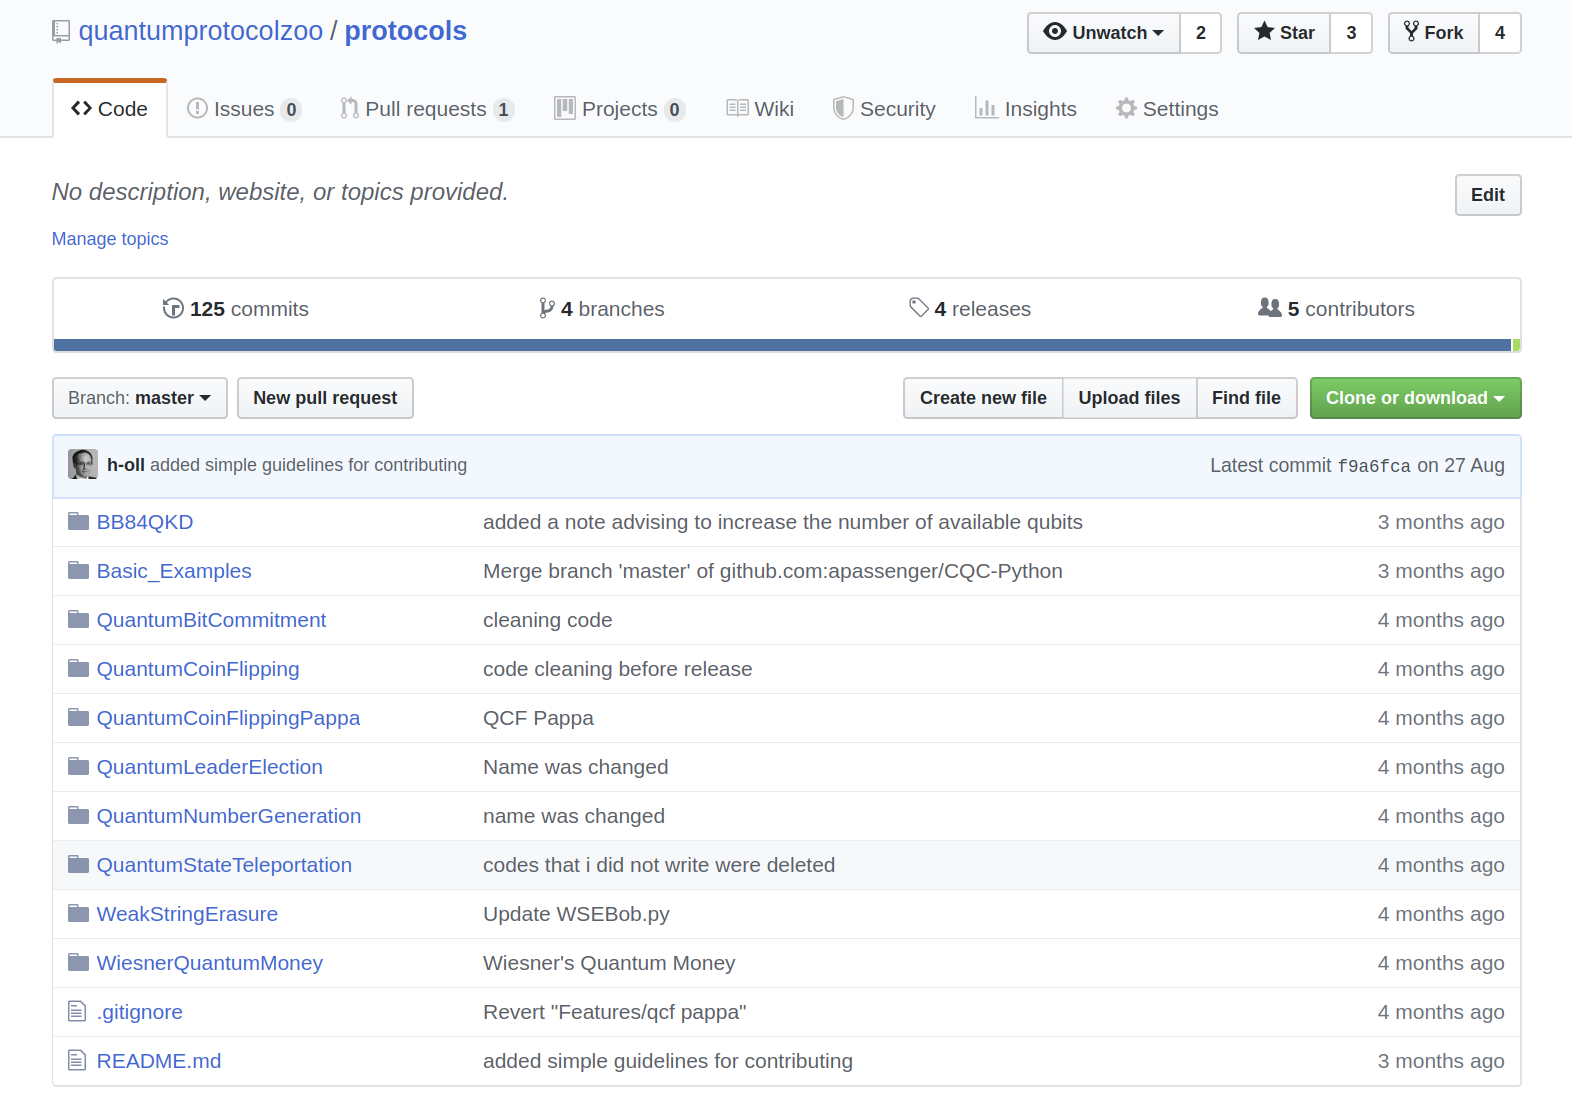
\includegraphics[width=.9\linewidth]{./figs/qpz_protocols.png}
\end{center}
\end{column}
\end{columns}

\begin{block}{}
\url{https://www.github.com/quantumprotocolzoo/protocols}
\end{block}
\end{frame}

\begin{frame}[label={sec:orgdd7e448}]{What's new: Certification library}
\begin{columns}
\begin{column}{0.4\columnwidth}
\begin{itemize}
\item 7 classes
\item 7 protocols described
\item 9 more being worked out
\end{itemize}
\end{column}

\begin{column}{0.6\columnwidth}
\begin{center}
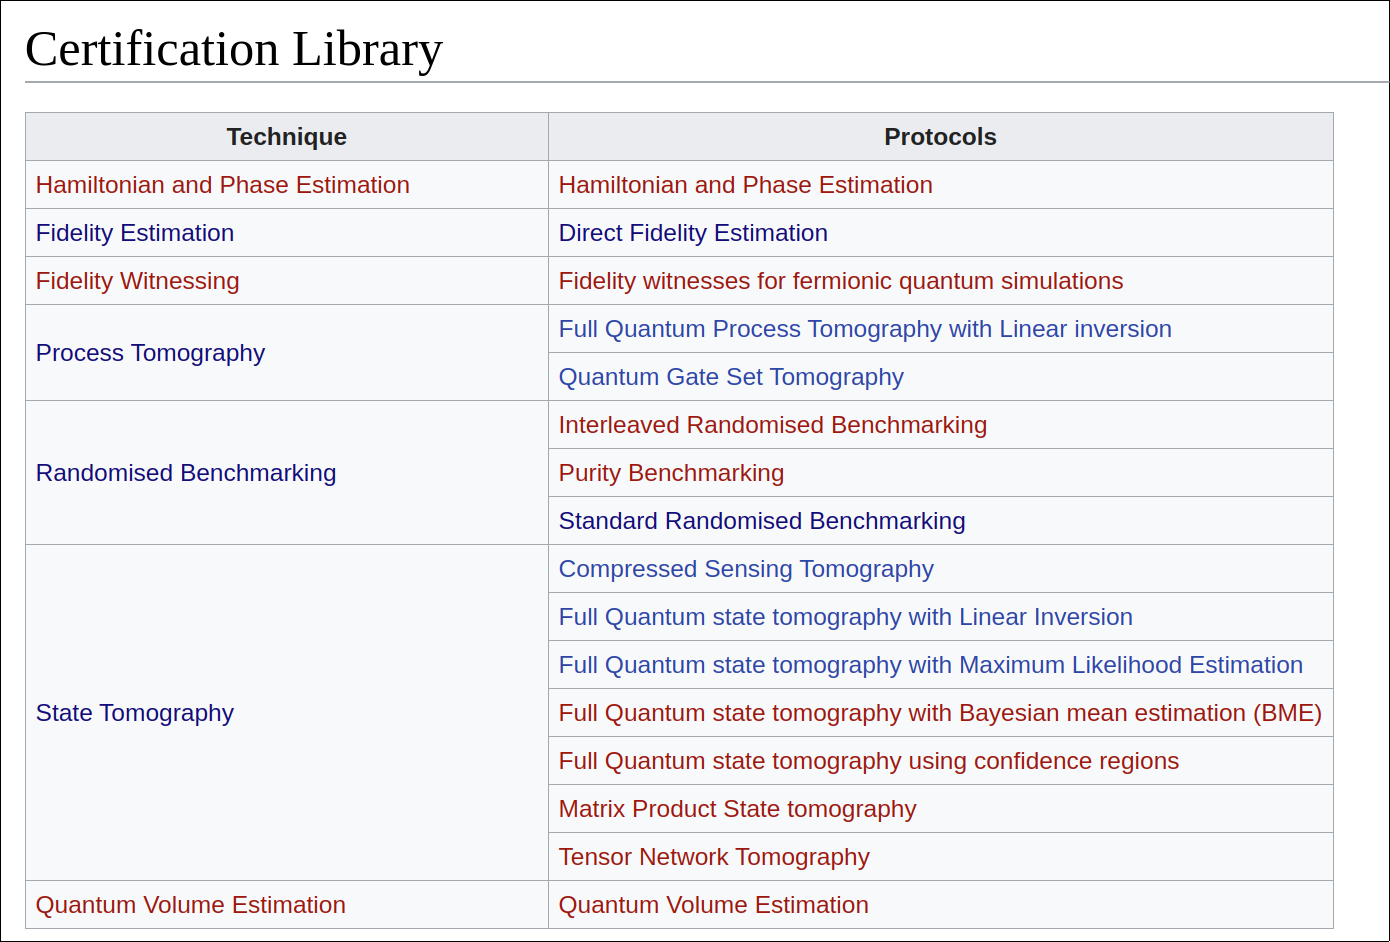
\includegraphics[width=.9\linewidth]{./figs/wiki_certification.png}
\end{center}
\end{column}
\end{columns}
\end{frame}

\begin{frame}[label={sec:org61b430c}]{What's new: Local information processing library}
\begin{columns}
\begin{column}{0.4\columnwidth}
\begin{itemize}
\item Planning a separate "local information processing" page
\item Distinguish comm. / cert. / local IP
\end{itemize}
\end{column}
\begin{column}{0.6\columnwidth}
\begin{center}
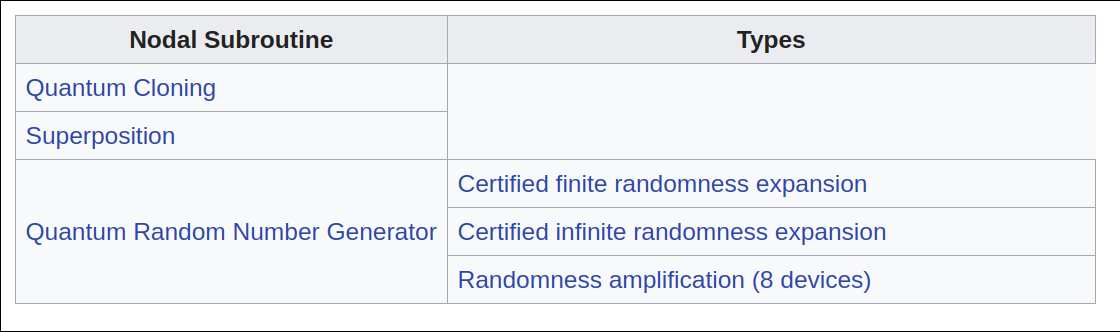
\includegraphics[width=.9\linewidth]{./figs/wiki_subroutines.png}
\end{center}
\end{column}
\end{columns}
\end{frame}
\begin{frame}[label={sec:orgac74c0d}]{What's new: 2-step submission process}
\begin{columns}
\begin{column}{.4\columnwidth}
\begin{itemize}
\item Each submission needs approval
\item Pages needing approval are visible to logged in users
\item Log in!
\end{itemize}
\end{column}
\begin{column}{.6\columnwidth}
\begin{center}
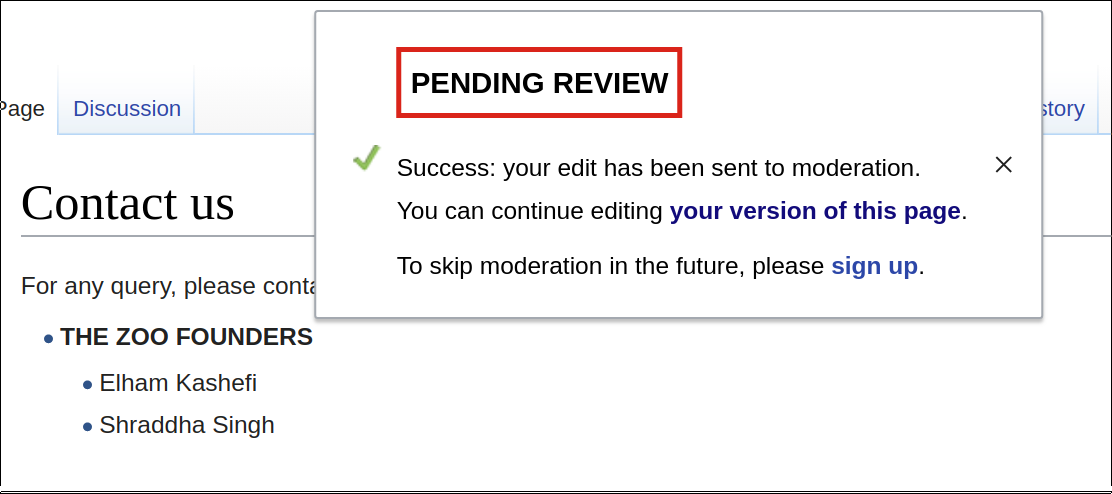
\includegraphics[width=.9\linewidth]{./figs/wiki_submission.png}
\end{center}
\end{column}
\end{columns}
\end{frame}
\begin{frame}[label={sec:org62134f8}]{What's new: Knowledge graph}
\begin{columns}
\begin{column}{.4\columnwidth}
\begin{itemize}
\item A page for exploring the full KG
\item A local KG per protocol
\item Single source of truth
\item Soon fixing the I-don't-see-what-I-should-do problem
\end{itemize}
\end{column}
\begin{column}{.6\columnwidth}
\begin{center}
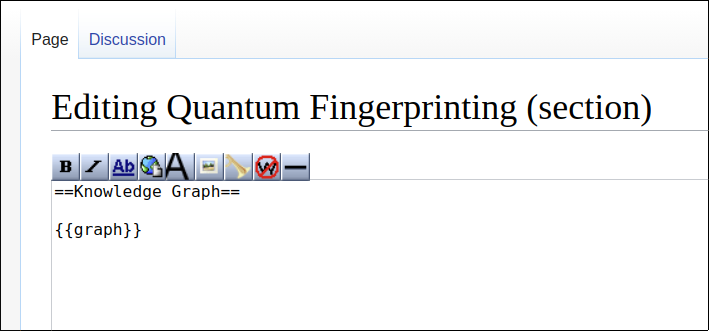
\includegraphics[width=.9\linewidth]{./figs/wiki_kg.png}
\end{center}
\begin{center}
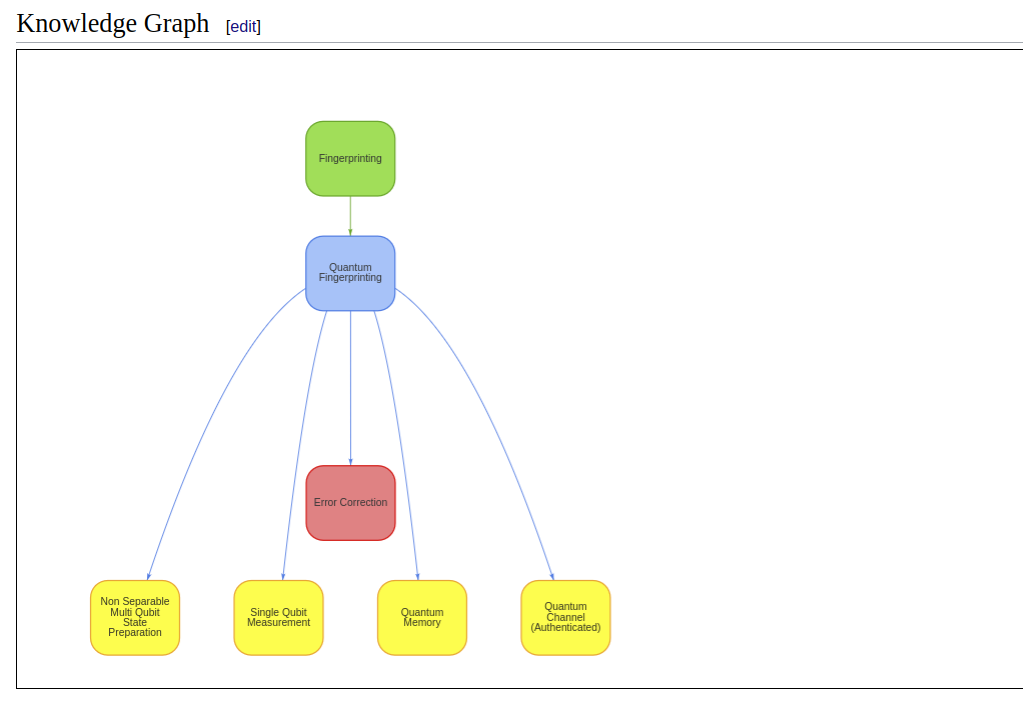
\includegraphics[width=.9\linewidth]{./figs/wiki_kg_2.png}
\end{center}
\end{column}
\end{columns}
\end{frame}
\begin{frame}[label={sec:org25bf850}]{What's new: Planning a new home page}
\begin{columns}
\begin{column}{.4\columnwidth}
\begin{itemize}
\item Short(er)
\item Shows what you can find
\item Visual
\end{itemize}
\end{column}
\begin{column}{.6\columnwidth}
\begin{center}
\includegraphics[width=.9\linewidth]{./draw_me_a_protocol.jpg}
\end{center}
\end{column}
\end{columns}
\end{frame}
\begin{frame}[label={sec:orge963a3e}]{What's new: What should you remember?}
\begin{columns}
\begin{column}{.6\columnwidth}
Contribute, promote, use!
\begin{itemize}
\item \url{https://wiki.veriqloud.fr}
\item \url{https://www.github.com/quantumprotocolzoo/protocols}
\end{itemize}
\end{column}
\begin{column}{.4\columnwidth}
\begin{center}
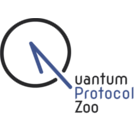
\includegraphics[width=.9\linewidth]{./figs/wiki_logo.png}
\end{center}
\end{column}
\end{columns}
\end{frame}


\section{Part II: Using the zoo}
\label{sec:orgd3834a9}
\begin{frame}[label={sec:org6896619}]{Part II: Using the zoo}
\end{frame}
\begin{frame}[label={sec:org4e67905}]{Using it: It works!}
\begin{columns}
\begin{column}{.4\columnwidth}
\begin{itemize}
\item 6 locations
\item About 80 participants
\item Impressive presentations
\end{itemize}
\end{column}
\begin{column}{.6\columnwidth}
\begin{center}
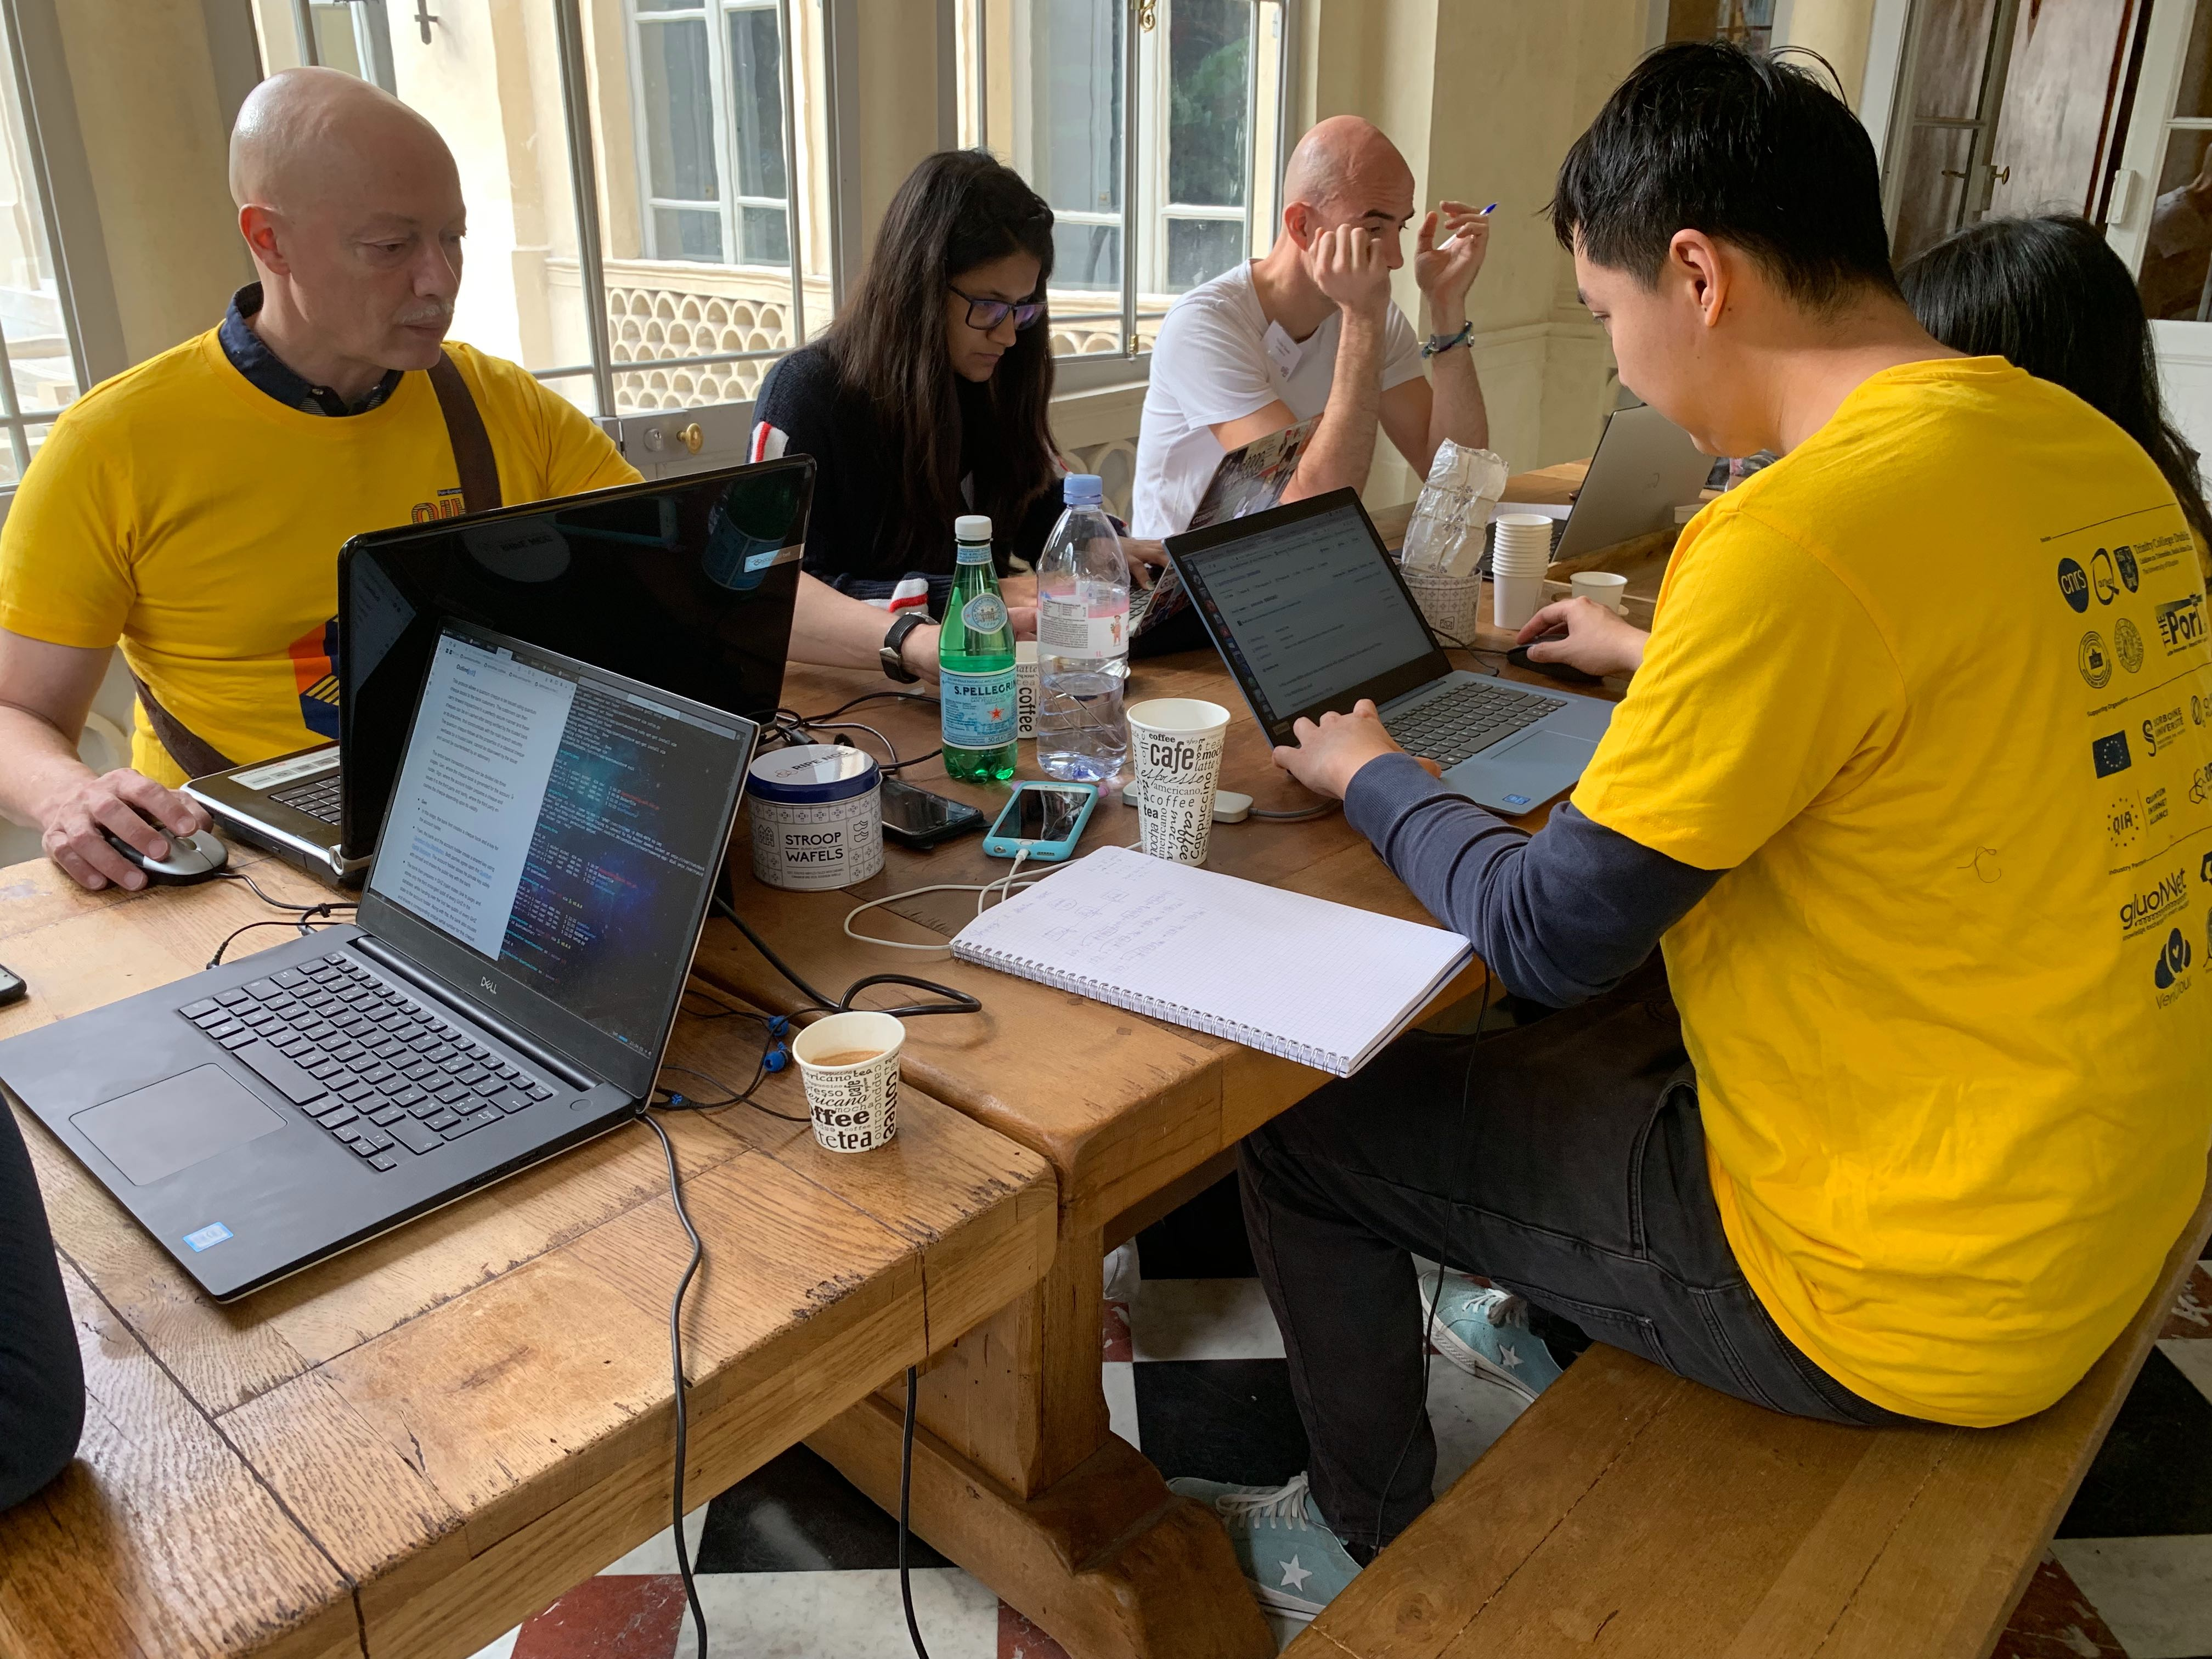
\includegraphics[width=.9\linewidth]{./figs/hackathon.jpg}
\end{center}
\end{column}
\end{columns}
\end{frame}

\begin{frame}[label={sec:org055c9e9}]{Using it: What did we learn?}
\begin{block}{It is useful}
\begin{itemize}
\item Enough to find the challenges
\item (Almost) enough to code
\end{itemize}
\end{block}
\begin{block}{It needs expansion}
\begin{itemize}
\item More protocols
\item More code (examples + higher-order functions)
\item More details (links to security proof, type of security achieved)
\end{itemize}
\end{block}
\end{frame}

\begin{frame}[label={sec:org424f4d6}]{Using it: Planning the future}
\begin{columns}
\begin{column}{.6\columnwidth}
\begin{block}{The "Delft" approach\ldots{}}
\begin{itemize}
\item Simulate
\item Build network layers on what you can do
\end{itemize}
\end{block}

\begin{block}{\ldots{} raises some challenges}
\begin{itemize}
\item Experimentalists want to know if they'll publish in Nature!
\begin{itemize}
\item Simulate or not simulate?
\end{itemize}
\item Reconciling the use of network model layers with security proofs
\begin{itemize}
\item Calling lower-layers for services implies decomposing protocols
\item Is it legitimate ?
\end{itemize}
\end{itemize}
\end{block}
\end{column}

\begin{column}{.4\columnwidth}
\begin{center}
\includegraphics[width=.9\linewidth]{./figs/network_stack.png}
\end{center}
\end{column}
\end{columns}
\end{frame}


\begin{frame}[label={sec:org3026cb4}]{Using it: Planning the future}
\begin{block}{Adopt a top-down approach}
\begin{itemize}
\item Applications is what matters
\item Proper services should be provided (experimentalists will know if it's worth working on a protocol)
\item Abstract crypto as much as possible (quantum networks should be secure by design)
\end{itemize}

\alert{\alert{Now better than later!}}
\end{block}
\end{frame}


\section{Part III: Going further}
\label{sec:orgec8f6e7}
\begin{frame}[label={sec:org6db556e}]{Part III: Going further}
\end{frame}

\begin{frame}[label={sec:org428e766}]{Direct link or teleportation ?}
\begin{itemize}
\item Protocols make use of direct links between players:
\begin{itemize}
\item Send qubit from \(A\) to \(B\)
\end{itemize}
\item Network stack is not planning to send qubits but to teleport them
\begin{itemize}
\item Is it working ?
\item Does it compose ?
\end{itemize}
\item And if it's OK doesn't it use sources of EPR pairs ?
\begin{itemize}
\item How do I get one ?
\item Are all implementations OK ?
\end{itemize}
\end{itemize}
\end{frame}


\begin{frame}[label={sec:org99a55ac}]{Constructing a Direct Quantum Link with Teleportation}
\begin{columns}[t]
\begin{column}{.5\columnwidth}
\begin{block}{Direct Quantum Link}
\begin{center}
\includegraphics[width=.9\linewidth]{./figs/direct_quantum_link.png}
\end{center}
\end{block}
\end{column}
\begin{column}{.5\columnwidth}
\begin{block}{Teleportation}
\begin{center}
\includegraphics[width=.9\linewidth]{./figs/teleportation.png}
\end{center}
\end{block}
\end{column}
\end{columns}
\end{frame}

\begin{frame}[label={sec:org888c50b}]{Teleportation correctly implements Direct Quantum Link}
\begin{columns}[t]
\begin{column}{.5\columnwidth}
\begin{block}{Direct Quantum Link}
\begin{center}
\includegraphics[width=.9\linewidth]{./figs/direct_quantum_link_filtered.png}
\end{center}
\end{block}
\end{column}
\begin{column}{.5\columnwidth}
\begin{block}{Teleportation}
\begin{center}
\includegraphics[width=.9\linewidth]{./figs/teleportation_filtered.png}
\end{center}
\end{block}
\end{column}
\end{columns}
\begin{block}{}
When no one is listening, teleportation works (perfectly)
\end{block}
\end{frame}

\begin{frame}[label={sec:org58dfed8}]{Teleportation securely implements Direct Quantum Link}
\begin{columns}[t]
\begin{column}{.5\columnwidth}
\begin{block}{Direct Quantum Link + simulator}
\begin{center}
\includegraphics[width=.9\linewidth]{./figs/direct_quantum_link_simulator.png}
\end{center}
\end{block}
\end{column}
\begin{column}{.5\columnwidth}
\begin{block}{Teleportation}
\begin{center}
\includegraphics[width=.9\linewidth]{./figs/teleportation.png}
\end{center}
\end{block}
\end{column}
\end{columns}
\begin{block}{}
Isn't it cheating? 

No! The Direct Quantum Link does not achieve any security; the simulator rightfully  gets the to-be-transmitted quantum state. 
\end{block}
\end{frame}


\begin{frame}[label={sec:orgeb323a0}]{Constructing a perfect EPR-source from Distillation}
\alert{\alert{Using a perfect EPR-source is no fun}}
\begin{columns}[t]
\begin{column}{.5\columnwidth}
\begin{block}{Perfect EPR-source}
\begin{center}
\includegraphics[width=.9\linewidth]{./figs/epr_source.png}
\end{center}
\end{block}
\end{column}
\begin{column}{.5\columnwidth}
\begin{block}{Distillation}
\begin{center}
\includegraphics[width=.9\linewidth]{./figs/distillation.png}
\end{center}
\end{block}
\end{column}
\end{columns}
\end{frame}
\begin{frame}[label={sec:org01db217}]{More on distillation (1/2)}
3-step process
\begin{itemize}
\item Apply Twirl + Symmetrisation
\item Verify that fidelity is what you expect or abort
\item Choose and apply a suitable distillation protocol
\end{itemize}
\end{frame}

\begin{frame}[label={sec:org2c7d2ac}]{More on distillation (2/2)}
\begin{itemize}
\item Initial state: \(\rho_{ABE} \in \mathcal{H}_2^{\otimes n} \otimes \mathcal{H}_2^{\otimes n} \otimes \mathcal H_E\)
\item Entering protocol: \(\rho = \text{Tr}_{E}(\rho_{ABE}) \in \mathcal H_2^{\otimes n} \otimes \mathcal H_2^{\otimes n}\)
\item Twirl + Symmetrisation: \(\rho_1 = \mathcal E_1(\rho) \in \mathcal H_2^{\otimes n-m} \otimes \mathcal H_2^{\otimes n-m}\)
\item Fidelity est.: \(\rho_2 = \mathcal E_2(\rho_1) \in \mathcal H_2^{\otimes n-m-l} \otimes \mathcal H_2^{\otimes n-m-l} \oplus \mathcal H_\perp\)
\item Distillation \(\rho_3 = \mathcal E_3(\rho_2) \in \mathcal H_2^{\otimes n-m-l-k} \otimes \mathcal H_2^{\otimes n-m-l-k} \oplus \mathcal H_\perp\)
\end{itemize}
\end{frame}

\begin{frame}[label={sec:org179e2c8}]{Distillation correctly implements a perfect EPR-source (1/2)}
\begin{columns}[t]
\begin{column}{.5\columnwidth}
\begin{block}{Perfect EPR-source}
\begin{center}
\includegraphics[width=.9\linewidth]{./figs/epr_source_filtered.png}
\end{center}
\end{block}
\end{column}
\begin{column}{.5\columnwidth}
\begin{block}{Distillation}
\begin{center}
\includegraphics[width=.9\linewidth]{./figs/distillation_filtered.png}
\end{center}
\end{block}
\end{column}
\end{columns}
\end{frame}
\begin{frame}[label={sec:org40a4bab}]{Distillation correctly implements a perfect EPR-source (2/2)}
\begin{itemize}
\item Twirl + Symmetrization
\end{itemize}
$$\rho_1 = \rho_{\text{source}}^{\otimes n-m}$$ 
\begin{itemize}
\item Finite precision fidelity estimation
\end{itemize}
$$\rho_2 \approx (1-p_\perp) \rho_W^{\otimes n-m-l}  + p_\perp \ket{\perp}\bra{\perp}$$ 
\begin{itemize}
\item Strictly positive rate distillation
\end{itemize}
$$\rho_3 \approx (1-p_\perp') \ket{\Phi^+}\bra{\Phi^+} ^{\otimes n-m-l-k} + p_\perp' \ket{\perp}\bra{\perp}$$
\end{frame}

\begin{frame}[label={sec:org6609ddd}]{Distillation securely implements a perfect EPR-source (1/3)}
\begin{columns}[t]
\begin{column}{.5\columnwidth}
\begin{block}{Perfect EPR-source + simulator}
\begin{center}
\includegraphics[width=.9\linewidth]{./figs/epr_source_simulator.png}
\end{center}
\end{block}
\end{column}
\begin{column}{.5\columnwidth}
\begin{block}{Distillation}
\begin{center}
\includegraphics[width=.9\linewidth]{./figs/distillation.png}
\end{center}
\end{block}
\end{column}
\end{columns}
\end{frame}
\begin{frame}[label={sec:org5d19fde}]{Distillation securely implements a perfect EPR-source (2/3)}
We should be looking at \(\rho_{ABE}\), but in fact we can get away by (almost only) looking at \(\rho_{AB}\)!

\begin{itemize}
\item Tracing out
\end{itemize}
$$\rho = \text{Tr}_E(\rho_{ABE})$$
\begin{itemize}
\item Twirl + Symmetrization
\end{itemize}
$$\rho_1 \approx \rho_{2\times 2}^{\otimes n-m}$$
\begin{itemize}
\item Finite precision fidelity estimation
\end{itemize}
$$\rho_2  \approx (1-p_\perp) \rho_W^{\otimes n-m-l}  + p_\perp \ket{\perp}\bra{\perp}$$ 
\begin{itemize}
\item Strictly positive rate distillation
\end{itemize}
$$\rho_3 \approx (1-p_\perp') \ket{\Phi^+}\bra{\Phi^+} ^{\otimes n-m-l-k} + p_\perp' \ket{\perp}\bra{\perp}$$
\end{frame}

\begin{frame}[label={sec:orgaaed667}]{Distillation securely implements a perfect EPR-source (3/3)}
We should be looking at \(\rho_{ABE}\), but in fact we can get away by (almost only) looking at \(\rho_{AB}\)!

\begin{itemize}
\item The analysis without \(E\) gives
\end{itemize}
$$( \mathcal{E}_3 \circ \mathcal E_2 \circ \mathcal E_1)  \text{Tr}_E \rho_{ABE} \approx (1-p_\perp') \ket{\Phi^+}\bra{\Phi^+} ^{\otimes n-m-l-k} + p_\perp' \ket{\perp}\bra{\perp}$$

\begin{itemize}
\item Gentle measurement theorem implies (because we are next to a \alert{pure} state when pairs are produced)
\end{itemize}
$$((\mathcal{E}_3 \circ \mathcal E_2 \circ \mathcal E_1) \otimes \text{Id}_E) \rho_{ABE} \approx ((1-p_\perp') \ket{\Phi^+}\bra{\Phi^+} ^{\otimes n-m-l-k} \\+ p_\perp' \ket{\perp}\bra{\perp})\otimes \text{Tr}_{AB} (\rho_{ABE})$$
\end{frame}


\section{Conclusion}
\label{sec:org903d847}

\begin{frame}[label={sec:orgfa0b704}]{Conclusion}
\begin{itemize}
\item We have a great tool to expand at \url{https://wiki.veriqloud.fr}
\item It's directly useful to the community and also to ourselves
\item Expand this kind of analysis
\begin{itemize}
\item Look at other elementary functions
\item Take noise into account
\end{itemize}
\end{itemize}
\end{frame}
\end{document}
